\documentclass{article}
\usepackage[utf8]{inputenc}
\usepackage{hyperref}
\usepackage{float}
\usepackage[table,xcdraw]{xcolor}
%\usepackage[sort&compress,square,comma,authoryear]{natbib}
\usepackage{booktabs}
\usepackage{graphicx}
\graphicspath{{Figures/}}
\usepackage{longtable}

\usepackage[
backend=biber,
style=authoryear,
sorting=nyt % sort by name year title
]{biblatex}
\addbibresource{Ref_invertebrate_DB.bib}

\title{ OUTLINE: Harmonized macroinvertebrate trait database, Aggregation of traits, Trait definitions, Sources }
\author{}%Stefan Kunz 
\date{}%June 2019


\begin{document}
%TODO: Use citep & citet instead of cite
\maketitle

\section{Introduction}

% !General introduction: Invertebrates importance/biodiversity and stressor
% ? use Traits mechanistic relationship, environmental filtering
% Half of all described freshwater invertebrates are aquatic insects

In the age of the Anthropocene invertebrates are exposed to multiple stressors such 
as chemical pollution, hydro-morphological modifications, invasive species and climate change. %?Sources 
Freshwater invertebrates play a crucial role for many ecosystem processes such as 
carbon cycling and water purification. In addition to their functional role, 10 \% of all 
described species live in freshwaters, most of which being invertebrates, and thus represent a
large part of animal biodiversity.
Understanding distributions of invertebrate communities and predicting effects of 
potential stressors is a long time goal of freshwater research. Since the 1970s 
ecologists have started using organismal traits to group aquatic insect species % ?to understand what -> Check Cummins

Traits are biological characteristics or ecological preferences measurable at the 
individual organism. %? Source Lancaster? Find precises definition
They reflect an organisms adaptation to its habitat. Trait based approaches in 
ecology are based on the habitat template theory, that predicts where environmental conditions
are similar trait composition should also converge, even across biogeographic boundaries. %?Source
Furthermore, several studies suggested that trait variability is lesser on larger geographical
scales than taxonomic variability %?Source Bonada 
Hence, trait based approaches can be a suitable tool for comparing the effect of various 
environmental stressors to invertebrate communities on large scales or across regions. 
%!General studies? Or more specific to studies for several regions
% They have been used to understand species distributions, in predicting effects of various environmental
% stressors to invertebrate communities, and as tool in biomonitoring. %? Source: Statzner & Beche 2010, Ralf Paper, Cummins Paper?
Consequently, studies have been carried out that e.g. examine the relationship between climate
and freshwater community assemblages using species traits. % TODO: Cite Bhowmik, cite Brown 
% TODO: Enrich with examples -> Maybe for toxicants as well?
Many of such studies combine information from several trait databases. For example, 
Brown et al. used in their study traits from invertebrate trait databases from
Europe, North America and New Zealand to investigate the effect of decreasing glacier cover
to river ecosystems. %TODO Cite Brown

% Studies that use information on aquatic invertebrate traits from different regions
% and/or aggregate trait information are increasing 
% !Transition into trait data
In fact, invertebrate trait data are increasingly available. Over the last decades aquatic 
ecologists have compiled comprehensive databases on invertebrate traits for different regions 
(see table \ref{tab:trait_databases} for examples). 
% !Mention various problems with trait databases 
However, researchers face various problems when the need to synthesize information from 
multiple invertebrate trait databases. 
% !Trait terminology
i) The use of inconsistent terminology across studies (see \cite{schmera_proposed_2015}
for a comprehensive discussion). 
For example, some studies used the term "trait" to describe a general 
organismal property like "generations per year" (\cite{statzner_reproductive_1997}, 
\cite{ussegliopolatera_biological_2000}), while in other studies this 
term was related to categories like "bi/multivoltine" 
(\cite{haybach_use_2004}, \cite{vieira_database_nodate}). Here, we follow 
the proposal of Schmera et al. (2015) and use the term \textit{trait} for a morphological,
physiological, or phenomenological feature measurable at the individual
organism (e.g. tegument, gills, etc.) and the term \textit{grouping feature} to describe 
a general property of related organismal traits (e.g. respiration). 
%? Include measurement scale?
%TODO: in concordance with previous paragraphs on trait definitions
%! Different traits used/definitions
ii) Invertebrate trait databases from different regions are not standardized. 
Often, the same grouping features are categorized using different traits. 
% TODO Example
This is complicated by the use of different measurement scales. For example, trait databases 
from North America use traditionally a binary coding (i.e. trait is expressed or not), 
whereas most other trait databases (e.g. Tachet, freshwaterecology, and New Zealand) 
use fuzzy coding (i.e. trait is expressed to a certain extent). 
Hence, transformation of nominal scale to ratio scale or vice versa is required. %? Wording
Furthermore, definitions for some traits differ as well across databases. 
% TODO Example feeding!
%! Taxonomical resolution & traits aggregation -> no guidance
iii) Taxonomical resolution between databases differs, further complicating the
synthesis of trait data from different regions. For example, some databases have recorded
trait information on mixed levels of taxonomical resolution like the North American trait
database or the Australian trait database. In contrast, trait information in the 
freshwaterecology database is entirely recorded on species-level. %?ref to graphic
%TODO: Percentages of different levels of taxonomical resolutions in process overview graph 
Using trait information on varying taxonomical levels is only possible when 
traits are aggregated to the lowest taxonomical level that is shared by all used databases. 
However, so far no one studied the effect of different trait aggregations 
Hence, iiii) guidance on how to perform a robust trait aggregation is missing. 
% TODO Poff Paper example, check Brown and other literature

%!Incentive of our analysis:
% no API/R packages 
Given the problems mentioned above extensive data processing is required before researchers 
can use multiple invertebrate trait databases for their work. 
In this paper we examine difficulties that ecologists face when synthesizing trait 
information from different invertebrate trait databases. We explore the effect of different
decisions researches have to make when working with invertebrate trait data 
from several sources, involving trait harmonization, handling different codings,
normalization, and aggregation of traits.
%?Effect of a statistical analysis -> Clustering?
%!What we did/Goal:
Therefore, we harmonized six grouping features of different trait databases from four
regions and aggregated the trait information to family-level. % ?Name Traits
We discuss the harmonization and show the effect of different ways of aggregating 
traits (inter alia Problem of different coding styles (fuzzy vs binary)).
We also present an overview of differences in trait definitions among databases.
Finally, our paper compares the references for the trait information that 
were specified in the trait databases we used.


%TODO: Change heading to be more expressive
\section{Description of harmonized trait database} 

% TODO Give a motivation (better in introduction?)
The harmonized database uses the available information on aquatic 
insect traits for the regions Europe, North America, Australia, and New Zealand. 
Due to the different number and identity of grouping features in each database, 
the following six grouping features were chosen for this study: locomotion, feeding mode, 
respiration, voltinism, size, and body form. 
The pattern of development (with the traits holometabolous or hemimetabolous) was added as
an additional grouping feature based on the orders of the taxa included in each database. 
% TODO: Few words why these grouping features have been selected
% TODO: Reasoning why no ecological grouping features have been used
Trait information for Australia and New Zealand were retrieved from 
a single database, respectively. For Europe we gathered trait information from the 
freshwaterecology trait database (\url{https://www.freshwaterecology.info/}) 
and complemented missing information with the 
Tachet trait database (\cite{usseglio-polatera_biomonitoring_2000}). 
North American macroinvertebrate traits were retrieved from Laura Twardochleb and 
complemented by trait information from Vieira et al (\cite{vieira_database_nodate}). 
We used all available information on invertebrates in the databases but restricted
our analysis to taxa that have complete trait profiles for the grouping features
mentioned earlier 
% !Short paragraph on imputation

% TODO: Insert citation
Table \ref{tab:trait_databases} gives an overview of the used databases. \\ 
In the following paragraphs, we describe the data processing steps required to 
establish a harmonized macroinvertebrate trait database. 

\begin{table}[H]
    \centering
    \caption{Overview of trait databases.}
    \label{tab:trait_databases}
    \begin{tabular}{lll}
    \toprule
   Region & Coding of trait states & Reference \\ 
    \hline
   Europe & Largely fuzzy & \cite{schmidt-kloiber_www.freshwaterecology.info_2015}\\ 
   Central Europe & Fuzzy coded & \cite{usseglio-polatera_biomonitoring_2000} \\ 
   North America & Largely binary & \cite{vieira_database_nodate}\\
   North America & Largely binary & cite Laura Twardochleb \\
   Australia & Binary \& fuzzy coding  & \cite{kefford_ben_AST_DB_2019}\\ 
   New Zealand & Fuzzy coded & \\ %TODO: Create entry for more recent NZ reference
    \bottomrule
    \end{tabular}
\end{table}


\subsection{Normalization \& data conversion}

% !Coding & Scale general
Traits in the used databases were either coded by fuzzy codes, binary coded or 
to a small extent coded as continuous variable (e.g. size). 
Fuzzy codes capture the variation (i.e. temporal or spatial) in a trait making them 
superior to binary coding. Fuzzy coding is often represented by assigning affinity 
scores to a taxon to express its preference to a certain trait. Usually, these 
scores range from 0 representing no affinity to an arbitrary maximum value (often 3) 
which represents high affinity. This type of coding uses the ratio scale
and not the ordinal scale as one might intuitively assume. In fact, the intention of the 
developers of this coding system was to convert affinity scores to percentages 
per trait, e.g. for a grouping feature with four traits affinity scores of 
\textit{5, 6, 2, 2} are equal to \textit{1/3, 2/5, 2/15, 2/15} or 
\textit{33.3 \%, 40 \%, 13.3 \%, 13.3 \%} (\cite{chevenet_francois_fuzzy_1994}).

% !Issues with coding & scale in the trait databases
Establishing a harmonized database required traits on the same measurement scale to 
enable comparability. However, in the used databases traits varied within and among databases 
in terms of measurement scale. 
This problem was particularly apparent in the Australian database which is a collection 
of seven trait databases. Thus, several grouping features occur multiple times but with 
traits that have different types of codings and ranges. 
For example, body size occurs as continuous variable, with traits that are fuzzy coded,
and also with traits that are binary coded. Hence, continuous variables needed to be converted to 
binary variables. Ranges of the fuzzy coded traits (0 - 3) and binary (0 - 1) traits needed to be 
normalized in order to be able to meaningfully allocate the same traits later on 
(e.g. allocating body size small from several sources).
Similarly, the type of coding for a grouping feature varied among the databases. %?give example
Furthermore, in some databases fuzzy coded information occurred in different ranges 
(e.g. from 0 to 3 and from 0 to 5 in the Tachet database, from 0 to 10 in the 
freshwaterecology database). 

% !How to circumvent aforementioned issues
First of all, categorical traits were dummy coded into binary variables and continuous
traits such as maximum body size were converted into binary traits. 
% TODO: traits from NOA data were converted to fuzzy codes by allocating at genus level using frequency on species level
For the Australian trait database we applied a range normalization by dividing each fuzzy
coded trait by its potential maximum value. Consequently, the values of each trait
were converted to a range from 0 to 1 which allowed allocating the same trait from various
sources in the next step. Implicitly, we assumed for binary variables that a value of 1 
for a particular trait corresponded to the maximum affinity for that particular trait. 

% !Issue of duplicate taxa
Furthermore, in the Australian, Tachet, and the North American databases duplicate taxon entries 
(either on species, genus or family level) existed that were amalgamated. 
In case duplicate entries contained contrasting information on the same trait state the median 
was taken. % ?What about zero's -> were disregarded

% !Normalization/Standardization 
Every trait within each grouping feature was standardized by the sum of all traits within 
this particular grouping feature per taxon to get percentages per trait which can be used to 
compare and harmonize taxa regarding their traits. %!Wording


% TODO Various preprocessing steps: Taxonomical corrections

% TODO a few words about spreadsheets etc?

\subsection{Harmonization of traits and taxa}
\begin{itemize}
    \item Harmonization process: See also Schmera 2015 et al 
    \item Differences in trait definitions
    \item Sources of traits
\end{itemize}

% !What is harmonization? & Why is it needed?
% The previous paragraphs described the data preparation steps needed in order to be able to harmonize
% aquatic insect traits. 
Harmonization of traits means amalgamating several similar traits into a single trait. 
It has to be undertaken when grouping features from different sources (e.g. different regions) are
used and the grouping features do not contain the same traits. 
For example, in our study for the grouping feature locomotion the lowest number of traits that occur
for all databases was in the New Zealand trait database ("Swimmer", "Burrower", "Crawler", "Sessil"). 
Hence, in all other databases locomotion traits have been allocated into these four traits (see \ref{fig:harmon_overview_1}
and \ref{fig:harmon_overview_2}).
% !Taxonomical harmonization
% Harmonization is crucial -> number of cases & comparability
%?Give an example -> Clusteranalysis

% !How was the harmonization done? -> technical aspect.
Grouping features that differed in their traits among databases have been harmonised by 
condensing the traits in such a way that in the end the same grouping features in all databases
consisted of the same traits.  
Thereby, traits were amalgamated based on ecological knowledge or expert judgment. %!Wording 
Our approach of harmonizing the traits of the used databases is outlined in figures 
\ref{fig:harmon_overview_1} and \ref{fig:harmon_overview_2}. 

% TODO: HArmonization for feeding mode AUS needs to be finished!
\begin{figure}[H]
   \centering
   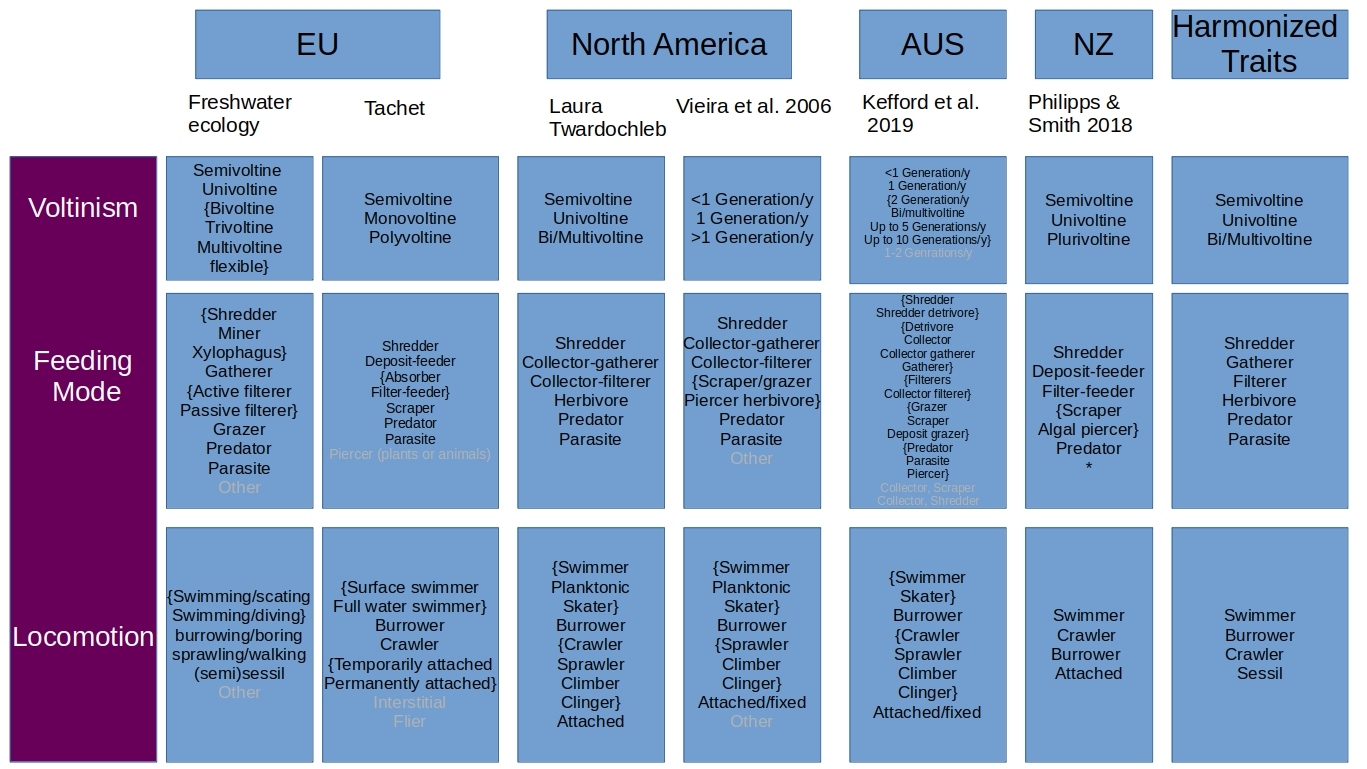
\includegraphics[width=16.5cm, height=10cm]{trait_overview1.jpg}
   \caption{Proposed harmonization scheme for the grouping features
   voltinism, feeding mode and locomotion. Shown are all traits for the 
   used grouping features in the investigated trait databases and 
   the harmonized traits in the end. Traits in curly brackets were 
   harmonized to one trait. Traits highlighted in Grey were omitted. \newline
   \textit{* Trait parasite was not available in New Zealand trait database.}
   }
   \label{fig:harmon_overview_1}
\end{figure}

\begin{figure}[H]
    \centering
    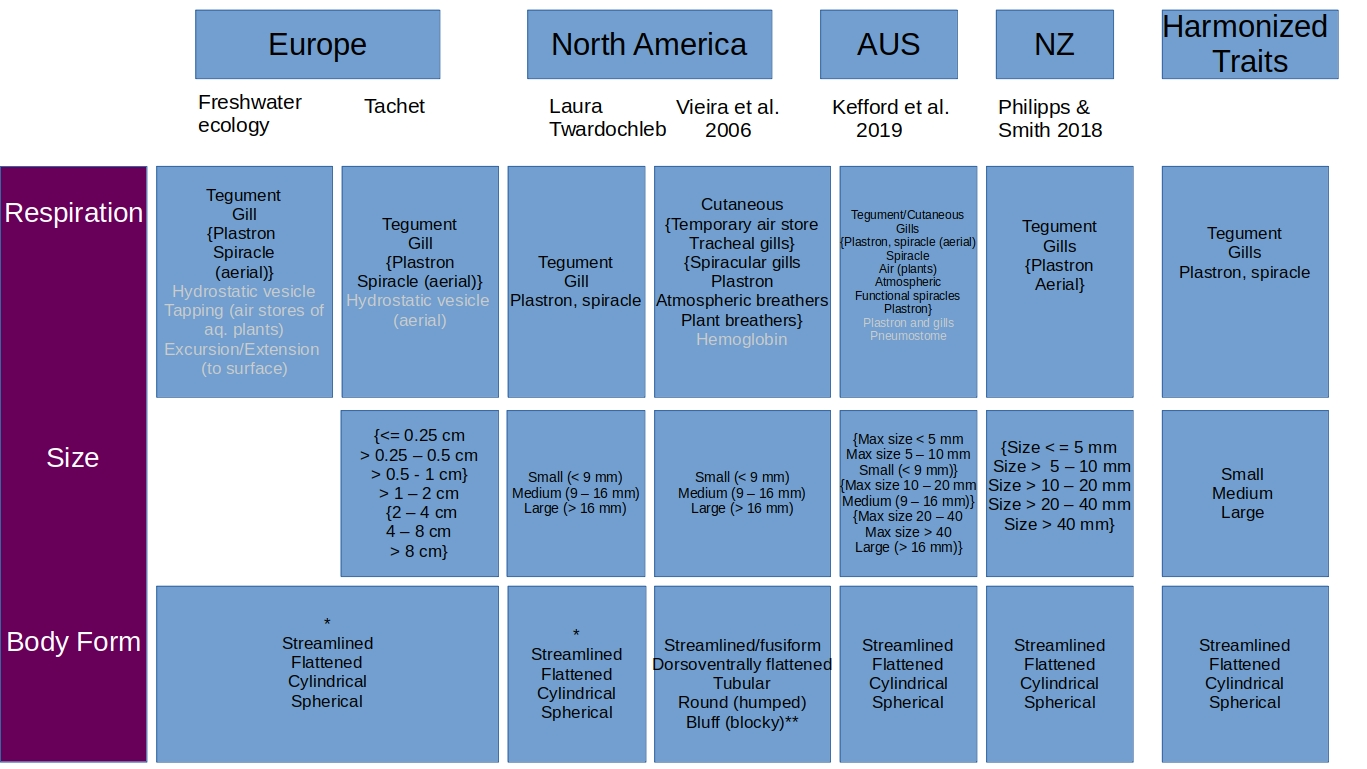
\includegraphics[width=16.5cm, height=10cm]{trait_overview2.jpg}
    \caption{Proposed harmonization scheme for the grouping features
    respiration, size and body form.\newline
    \textit{* Body form information provided by Philippe 
    Usseglio-Polatera.}\newline
    \textit{** Bluff(blocky) taxa have been reclassified
    by Philippe Usseglio-Polatera using the traits streamlined,
    flattened, cylindrical and spherical.} }
    \label{fig:harmon_overview_2}
 \end{figure}

% TODO: Go deeper -> Trait definitions
% !Trait harmonization subjective & always dangerous
Not only the categorization of grouping features but also the definitions of 
individual traits vary between databases, complicating harmonization. 
% TODO: Present definition comparison -> For all traits?

\section{Aggregation of traits}
% TODO Describing \& testing different approaches
% TODO Problem of coding of traits
%! Why would one want to aggregate traits?
% See Poff paper 

Two approaches were employed. 1) we used the preprocessed trait databases and 
aggregated taxa from species level to family level by allocating them at the genus 
level using the median. Then traits on genus-level were aggregated to
family-level by using the mode. In cases where it was not possible to take the mode 
(e.g. only distinct values or trait values like "1,1,2,2,3") the median was taken as well. 
% TODO improve example
2) we directly aggregated taxa to family level using the median.

Finally, the resulting aggregated trait values were compared to traits assigned at 
family level by experts. Those expert assignments on family level were not available for 
all databases nor for all traits assigned. Hence, we restricted our analysis to ...
% TODO: Comparison with traits assigned at family level for AUS & 
% TODO North America (on subsets only possible) -> Find suitable subet
% TODO: ATM done with all Taxa, just subset to Species data (does this make sense?)

\section{Results}
% TODO: For Results & Discussion taxonomic overlap between databases rather small

%%%%%%%%%%%%%%%%%%%%%%%%%%%%% MAIN RESULTS %%%%%%%%%%%%%%%%%%%%%%%%%%%%%
% Data preparation complex -> many decisions
% Databases are not ideal (not standardized, different trait definitions)
% Effect of trait aggregation
% Trait values only slightly vary between complex and direct aggregation
 % -> compare with family assignments: Roughly 25 % are classified differently
    % -> Which and why? 
    % -> Add statistical technique -> Maybe clustering?  
 % -> test with weights?
 % -> (effect of transforming binary to fuzzy codes -> US data subset test)
%%%%%%%%%%%%%%%%%%%%%%%%%%%%% MAIN RESULTS %%%%%%%%%%%%%%%%%%%%%%%%%%%%%


\section*{Additional ideas}

Section Description of databases:
\begin{itemize}
    \item Describe different databases briefly?
    \item State goal of analysis $\rightarrow$ reference to second paper?
\end{itemize}

\end{document}